\chapter[Estado del arte]{Estado del arte}
\label{ch:estado_del_arte}

\section{Reconocimiento de patrones}
\label{sec:rec_patrones}
	No existe una definición universalmente aceptada para el Reconocimiento de Patrones (RP). Esta puede recibir distintas definiciones dependiendo de la disciplina sobre la cual se quiere aplicar. Algunos autores como Duda et. al~\cite{Duda1973} definen el reconocimiento de patrones, junto con reconocimiento de máquina como un campo preocupado de las regularidades del ruido en entornos complejos. Sergios Theodoridis~\cite{Theodoridis2008} lo define como una disciplina científica que apunta a la clasificación de objetos dentro de un conjunto de categorías o clases, y también como una parte integral del sistema de inteligencia de la máquina construida para la toma de decisiones. Thomas González~\cite{Gonzalez1978} define RP como la clasificación de la entrada de datos a través de la extracción de importantes características de un conjunto de estos con ruido. 

\begin{figure}[b]
  \centering
   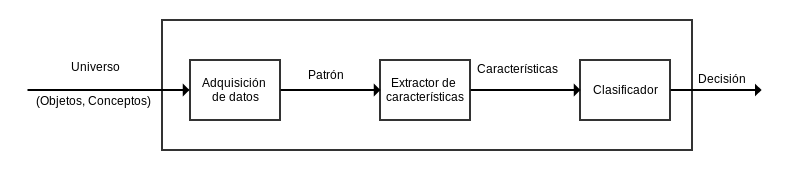
\includegraphics[width=1\textwidth]{Figuras/Diagramas/estado_del_arte/Reconocimiento_de_patrones.png}
  \caption{Arquitectura básica de un sistema de reconocimiento de patrones}
  \label{art:fig:arquitectura}
\end{figure}


En este trabajo se define el reconocimiento de patrones como un área de la Inteligencia Artificial (IA) enfocada en la extracción de características de un conjunto de imágenes o vídeos, las cuales definen los patrones que serán utilizados para la creación de un modelo que permita clasificar nuevas entradas. Podemos describir este procedimiento en tres procesos como se puede ver en la Figura~\ref{art:fig:arquitectura}: adquisición de datos, extracción de características y toma de decisiones. 

Existen diversos métodos que permiten solucionar el problema de clasificación, entre los cuales se encuentran las Máquinas de Vectores de Soporte~\cite{Cortes1995}~\cite{Hearst1998}.

	\paragraph{Máquinas de vectores de soporte}
	\label{sec:svm}
	Las máquinas de vectores de soportes (SVM sus siglas en inglés) son herramientas fundamentales en sistemas de aprendizaje automático, se basan en  implementar reglas de decisión complejas, por medio de un kernel que permite mapear los puntos de entrenamiento a un espacio de mayor dimensión. Estas máquinas son utilizadas para la clasificación y análisis de regresión permitiendo generar un modelo de predicción dado un conjunto de datos de entrada, y posteriormente utilizar este modelo para clasificar nuevos datos.
La idea del SVM es solucionar un problema de clasificación de dos clases mediante una barrera de decisión. Estos métodos evolucionaron con el tiempo y se utilizan para poder solucionar el problema de clasificación de múltiples clases.

Para efectos de este trabajo, SVM es utilizado para poder generar el modelo final que permita clasificar las seis expresiones faciales canónicas, utilizando los descriptores obtenidos luego de la extracción de características.

\section{Reconocimiento de expresiones faciales}
\label{sec:fer}
Las expresiones faciales constituyen una guía básica en la interacción social. Por ello, las alteraciones en su expresión o reconocimiento suponen una importante limitación para la comunicación. Ya que las expresiones del rostro son la variable que más se observa para obtener información de las emociones de nuestros interlocutores; si bien es cierto que tenemos un elevado control sobre nuestra expresividad facial, diversos estudios han demostrado que, cuando una persona está utilizando una expresión facial no acorde con su verdadero estado de ánimo, en su cara aparecen durante breves momentos señales de la emoción verdadera, que a menudo pasan desapercibidas para los demás.
El reconocimiento de expresiones faciales lo podemos dividir en dos grandes tipos: la extracción de características geométricas y extracción de características de apariencia, a su vez puede estar enfocado en reconocer las expresiones tanto en imágenes como en vídeos.  


\subsection{Expresiones faciales canónicas}
\label{sec:type_fe}
Dado que el rostro humano tiene una infinita variedad de posibles expresiones, Ekman estableció seis expresiones base o canónicas~\cite{Ekman1981}, las cuales son excluyentes entre sí, además de una expresión neutra. Las cuales son: Sorpresa (Surprise), Felicidad (Happiness), Tristeza (Sadness), Miedo (Fear), Cólera (Anger) y Asco (Disgust).


\subsection{Métodos basados en características geométricas}
\label{sec:met_geo}

\subsection{Métodos basados en características de apariencia}
\label{sec:met_apa}

	\subsubsection{Métodos sobre imágenes}
	\label{sec:met_imagen}
	

		\paragraph{Local Binary Patterns.}
		\label{sec:lbp}
		Método introducido por Wang y He~\cite{Wang1990}, consiste en realizar una codificación del píxel de interés con respecto a los valores de sus vecinos. En simples palabras se realiza un proceso de máscara en el cual se restan los píxeles del vecindario con el píxel central, si la resta es negativa o cero se asigna un cero en la posición del vecino, por el contrario si es positiva se asigna un uno. Luego de esto, se realiza una concatenación de los vecinos y se obtiene un código binario que es transformado a base 10. Dicho número es asignado como nuevo valor del píxel visitado~\cite{Ojala1994}, \cite{Ojala2002}, \cite{Ahonen2004}, \cite{Shan2009}.

Luego de realizar el proceso en todos los píxeles se procede a realizar un histograma de los valores el cual es definido como el descriptor de la imagen, siendo este utilizado una para posterior clasificación~\cite{Ahonen2006}.

Otros métodos que utilizan LBP antes de la obtención del descriptor dividen la imagen en $n$ secciones de igual o distintas áreas, y realizan el cálculo del histograma para cada una de estas secciones. Luego concatenan cada uno de los histogramas en un orden específico y se obtiene un macro descriptor más detallado de la imagen.

		\paragraph{LND}
		\label{sec:lnd}

	\subsubsection{Métodos sobre imágenes dinámicas}	
	\label{sec:met_videos}

		\paragraph{Volume Local Binary Patterns.}
		\label{sec:vlbp}
		Método introducido por Zhao y Pietikäinen~\cite{Zhao2006}, basado en LBP para imágenes dinámicas, el cual se basa en tres variables: $L$ la cantidad de cuadros que entran en la creación del patrón, $P$ el tamaño del vecindario a seleccionar y $R$ el radio del cual se escogen los vecinos. 
El método VLBP consiste en realizar una codificación basada en LBP, ahora incluyendo la variable temporal $L$ que indica desde qué cuadro se comienza a realizar la resta del píxel seleccionado con el central.
Éste es un proceso muy costoso debido a que mientras mayor sea la cantidad de vecinos a seleccionar, mayor será la cantidad de dígitos binarios, lo cual implica un mayor espectro de números resultantes en la codificación~\cite{Zhao2007a}, \cite{Zhao2007}.

		\paragraph{Local Binary Patterns-Three Ortogonal Planes}
		\label{sec:lbp-top}
		 Es un método basado en LBP para imágenes dinámicas, consiste en crear tres planos ortogonales que se intersectan en el píxel de interés, siendo estos el plano $XY$ , $XT$ y $YT$ (cuadro actual , movimiento temporal en $X$ y en $Y$ respectivamente). 

Para poder obtener el patrón de la imagen se realiza el mismo proceso de resta con los píxeles del vecindario seleccionado, pero a diferencia de los métodos estáticos que solo se realizan en el plano $XY$, este también se realiza para los planos $XT$ e $YT$.\@ Con esto se obtiene un histograma para cada plano, los cuales son concatenados y forman el macro descriptor de la imagen~\cite{Zhao2007}.


\section{Reconocimiento de rostros}
\label{sec:rec_rostros}

	\subsection{Viola-Jones}
	\label{sec:viola-jones}

\section{Optical flow}
\label{sec:optical_flow}

\section{Bag of words}
\label{sec:bag_of_words}

	\subsection{K-means}
	\label{sec:k-means}
	
	\subsection{Métricas de distancia}
	\label{sec:matricas_de_distancia}